%% bare_jrnl.tex
%% V1.4b
%% 2015/08/26
%% by Michael Shell
%% see http://www.michaelshell.org/
%% for current contact information.
%%
%% This is a skeleton file demonstrating the use of IEEEtran.cls
%% (requires IEEEtran.cls version 1.8b or later) with an IEEE
%% journal paper.
%%
%% Support sites:
%% http://www.michaelshell.org/tex/ieeetran/
%% http://www.ctan.org/pkg/ieeetran
%% and
%% http://www.ieee.org/

%%*************************************************************************
%% Legal Notice:
%% This code is offered as-is without any warranty either expressed or
%% implied; without even the implied warranty of MERCHANTABILITY or
%% FITNESS FOR A PARTICULAR PURPOSE! 
%% User assumes all risk.
%% In no event shall the IEEE or any contributor to this code be liable for
%% any damages or losses, including, but not limited to, incidental,
%% consequential, or any other damages, resulting from the use or misuse
%% of any information contained here.
%%
%% All comments are the opinions of their respective authors and are not
%% necessarily endorsed by the IEEE.
%%
%% This work is distributed under the LaTeX Project Public License (LPPL)
%% ( http://www.latex-project.org/ ) version 1.3, and may be freely used,
%% distributed and modified. A copy of the LPPL, version 1.3, is included
%% in the base LaTeX documentation of all distributions of LaTeX released
%% 2003/12/01 or later.
%% Retain all contribution notices and credits.
%% ** Modified files should be clearly indicated as such, including  **
%% ** renaming them and changing author support contact information. **
%%*************************************************************************

\documentclass[journal]{IEEEtran}
\usepackage{pgfplots}

\ifCLASSINFOpdf
  %\usepackage[pdftex]{graphicx}
  % declare the path(s) where your graphic files are
  %\graphicspath{{img/}}
  % and their extensions so you won't have to specify these with
  % every instance of \includegraphics
  %\DeclareGraphicsExtensions{.jpg,.pdf,.jpeg,.png}
\else
  % or other class option (dvipsone, dvipdf, if not using dvips). graphicx
  % will default to the driver specified in the system graphics.cfg if no
  % driver is specified.
  % \usepackage[dvips]{graphicx}
  % declare the path(s) where your graphic files are
  % \graphicspath{{../eps/}}
  % and their extensions so you won't have to specify these with
  % every instance of \includegraphics
  % \DeclareGraphicsExtensions{.eps}
\fi
\hyphenation{op-tical net-works semi-conduc-tor}


\usepackage{soul, color}

\begin{document}
\title{Implementation of a Non-Blocking\\ Hashtable using C++11}
\author{Timothy~Flowers,
        Austin~Lasher,
        and~Joseph~Maag% <-this % stops a space
}

\markboth{UCF COP4520 -- Parallel Processing, Assignment 2}
{Shell \MakeLowercase{\textit{et al.}}: Bare Demo of IEEEtran.cls for IEEE Journals}
\maketitle

\begin{abstract}
In the paper “Non-blocking Hashtables with Open Addressing”, Chris Purcell and Tim Harris propose a non-blocking hashtable that utilizes buckets, probe bounds, and open addressing for standard hashtable functionality and achieves non-blocking behavior with the use of atomic operations and custom word types. We implemented a sequential version of the proposed hashtable in a C++11 class that shares the core hashtable implementation but eliminates much of what makes it parallel. Our implementation was tested over a series of trials and resulted in a degradation of performance if the number of insertions and deletions were significantly higher than the number of search operations.
\end{abstract}

\section{Introduction}
\IEEEPARstart{I}{n} this paper we will describe a  sequential version of a non-blocking hashtable described by Chris Purcell and Tim Harris in their paper “Non-blocking Hashtables with Open Addressing”. We implemented the data structure a a C++11 class and performed a series of tests to assess its performance.
To describe our implementation and test results, we will first in Section 1 briefly describe the hashtable proposed in the original paper. Section 2 will describe the details of our C++11 sequential implementation of the hashtable. Lastly, we will describe our performance tests and analyze the results to give an overall view of the efficiency of a sequential version of the described hashtable.


 
\section{Algorithm Description}

The Non-Blocking implementation of our Hashtable contains three operations: Insert, Delete, and Contains. The function of these operations is described below, as well as a description of the necessary changes for a Non-Blocking implementation.

\subsection{Insert}
In order to insert into the table, the hash value must first be obtained. Starting from the bucket corresponding to the hash value, continue quadratic probing until they find a bucket that contains an EMPTY\_FLAG value. If the number of probes to get to that slot was greater than the upper bound stored for the inserted item's hash value, the upper bound should be updated to the number of probe jumps used to reach the EMPTY slot. Otherwise, the probe bound should remain unchanged. If at any point the number of probe jumps exceeds the size of the hash table, the function should return false to signal that the collision was unresolved and the insert operation failed.

\subsection{Remove}
In order to remove an element from the table, the hash value for the element must first be obtained. Starting from the bucket corresponding to the hash value, continue probing until the element is found or the upper bounds are exceeded. If the upper bound is exceeded return false to signal that the item was unable to be removed. If the item is found set the bucket its located in to EMPTY. If the number of probe jumps it takes to get to the bucket is equal to the upper bounds of the hash value, decrement the upper bound until probing by the number contained within the upper bound results in a non-empty bucket, or the upper bound equals zero.

\subsection{Contains}
In order to check for an element in the table, the hash value must first be obtained. Then starting from the bucket corresponding to the hash value, probing should continue until the upper bound of the hash value is exceeded or until the element to be searched for is found. If the element is found return true. Otherwise, if the bounds are exceeded, return false.


\section{Implementation}

Our C++11 implementation of the sequential hashtable data structure has many similarities to the structure and pseudocode described by Chris Purcell and Tim Harris, but has several changes to keep it sequential while utilizing the features of C++11.

\subsection{C++11}
The structure is encapsulated in a C++ class called NBHashTable with a standard C++ class source file ‘NBHashTable.cpp’ and header file ‘NBHashTable.h’. C++11 was chosen as our implementation language so we could utilize the thread support library that is part of the C++11 standard library. NBHashTable utilizes a ‘std::mutex’ object from the thread library to guarantee thread-safety. ‘std::thread’ objects are used in our main test classes to spawn threads and have them interact with a NBHashTable object.

\subsection{Buckets and Probe Bounds}
The internal storage structure of NBHashTable is an integer array ‘buckets’ that represents the hashtable bucket locations. The size of the array is determined by an integer argument passed into the NBHashTable constructor method. This value is assigned to an internal size variable ‘kSize’ and is used throughout the hashtable class, including for the instantiation of the buckets array. In our current implementation the variable is not constant, which will be necessary for making our hashtable resizable in the future.

Initially the bucket array locations are initialized to the value of the preprocessor macro 'EMPTY\_FLAG' defined in the NBHashTable header file. In our implementation it is set to -1 to represent an empty bucket. It is assumed only integers greater than -1 will be placed into buckets except when a value is removed from a bucket, in which case it is set back to the empty flag value -1.

The bounds values associated with each bucket location are represented as an integer array initialized to be the same size as the buckets array. Each location in the array is initially initialized to 0 to represent 0 collisions at each bucket location.

\subsection{Public Methods}
The public methods to ‘put’ and ‘remove’ values in NBHashTable have arguments of type NBType. NBType is defined in the header file as a typedef integer type. This type is used as an alternative to a standard ‘int’ to make possible changes to this type easier in future development.

Before each addition or removal of an integer value, the value is passed into a hash function to make an associated index that is within the range of this buckets and bounds array. This hash function is simply '(value \% kSize)' where kSize is the hashtable size.

The methods used to interact with the buckets are similar to those described in the paper, with one method to obtain values from the bucket, and one method to test whether a given collision exists. Both take a ‘startIndex’ integer argument representing the hashed version of an integer value to be added or removed, and a ‘probeJumps’ integer representing the length of the probe sequence needed to find the value. A pointer to a bounds location is returned when getting a bucket value so that the value can be changed without having to access the the bucket array twice. While not entirely necessary for our sequential implementation, this will be useful if we need to parallelize NBHashTable in the future.

When inserting or removing a value from the hashtable, the value is first hashed with the has method and is used as the first index location in the buckets array that is checked. When inserting, if there is already a value in that position in the array, other locations in the area are checked to be empty to find a location where it can be inserted instead. The locations checked in this probing sequence are determined by the quadratic formula '(startIndex + (probeJumps * (probeJumps + 1)) / 2'. This probing is executed in a for-loop with a counter called ‘probeJumps’, which is iterated until it is greater than the kSize constant or an empty location is found at an index defined by the quadratic equation.

When removing or locating an item, the same probing sequence is used, except the for-loop stops when the counter is greater than the bounds value at the original hash value location (or when the value it is searching for is found first).

As described in the paper, bound values are incremented with the addition of values whose collision value is greater than the hash indexes original value in the bounds array. A bound value is decremented with the removal of a value last in a probing sequence. The method ’conditionallyLowerBound’ is responsible for calculating and setting a new bounds uses a loop to search the probe sequence in reverse until it reaches a non-empty bucket, and then sets a new probe value at the original hash index.

\subsection{Sequential Modifications}
To keep the algorithm parallel and lock-free, the pseudocode provided uses lock-free atomic compare-and-swap functions when accessing and modifying bucket and bounds values. The paper also specifies packing a state, a version count, and a bucket value into a single word value for each bucket for atomic access and modification. The paper also suggests using a single word value that contains a scanning bit and a bounds value for each bounds value.

These modifications make the structure lock-free and parallel, so our implementation does not use them in order to keep the structure sequential. Bucket and bounds values are simply integer values that represent the bucket value, without any additional state values. Reads and writes to the bounds and buckets arrays are done directly without atomic operations. To keep the structure sequential and thread-safe, we use a single std::mutex object that is locked for every public method call and unlocked at the end of every public method. Even though this allows blocking and eliminates the non-blocking nature of the proposed hashtable, this guarantees only one public method can be executed at a time so that no two threads will be interacting with the hashtable at the same time. If one thread is interacting with the hashtable and another thread attempts to call one of its public methods simultaneously, it will have to wait until the first thread is finished. At this point, the holding thread will unlock the mutex, and a waiting thread will begin its interaction by locking it. Because NBHashTable public methods cannot execute simultaneously, sequential performance is guaranteed.

\section{Testing and Performance}

To compare our algorithm to the original description, we set up several testing suites that implemented our NBHashTable class. In the previous assignment, we focused on both correctness, and execution time. This time around, as we have added some additional structures to support non-sequential loads, we required several new tests in addition to the previous tests.

The first new test is our Atomic Types test file, "atomictypes.cpp". This program allowed us to create test cases for our ProbeBound and VersionState classes. As the paper showed, we used a bit-stealing technique to combine the probe bound and scanning bit into a single memory word, so a single compare-and-swap operation could update this value. The same process needed to be done for the Version and bucket state variables, except the bucket state required three bits as there were six possible states.

The second new test file is titled "instructions.cpp", and allows us to input exact numbers we wanted inserted and deleted. This way, we can set up even more specific tests and make sure that each function was working appropriately. These are input using standard input, so files can be piped as input to the program.


\subsection{Correctness}

Correctness is difficult to measure for all cases. Unlike execution time, it would be difficult to create a testing suite to measure correctness that randomly generates numbers. It would randomly have to generate insertions and deletions of numbers, and from that compare it to a "correct" output, that it would also have to generate. How can we be sure that the output it created was actually correct for every case? There is no way to be sure, as there could be a fault in our procedure that generates a "correct" output. A false positive, in this case, would be likely.

Our approach to measuring the correctness of the algorithm, instead, was to create several test cases. The idea is that we can create test cases, and compare the actual result to an expected result we retrieved on paper. With this method, we can create many different tricky test cases, and see how they perform individually. From each tricky test case, we were thereby able to refine our implementation to be certain of its correctness, and kept refining different portions of code until we were certain it was correct.

We have included our sample test cases in our initial submission document, under 'correctness1.cpp' and 'correctness2.cpp'. These can be built using our makefile with the target "make correctness". This will make two corresponding executables, correctness1 and correctness2 under the build/ directory. These can be run to show our testing methodology, and the proof of our algorithm can be visually seen.

\subsection{Execution time}

Execution time is important to test because it allows us to compare the specific operations of the algorithm and determine how it should be used most efficiently. It also allows us to compare our implementation to the expected time from the original paper, and potentially see the limits of our currently sequential solution.

Our goal is to measure execution for a potentially random set of data in bulk, and measure the approximate execution time depending on the number of threads. We also hope to visually see a correlation between the number of operations performed and the resulting execution time for those set of operations. To do this, we created a C++ program (executiontime.cpp) that we can run multiple times with different parameters, and will show the average execution time on the given parameters.

With this goal in mind, we approached the program by spawning some number of threads, and performed 500,000 operations on each of those threads. These were either insert() operations, delete() operations, or contains() operations. The distribution of each of these was modified into six different cases, shown in Table 1 below.

\begin{table}[h]
\centering
\begin{center}
\begin{tabular}{ |c|c|c|c| } 
 \hline
 Trial \# & insert() & delete() & contains() \\ 
 \hline
 1 & 75\% & 25\% & 0\% \\ 
 2 & 25\% & 75\% & 0\% \\ 
 3 & 50\% & 50\% & 0\% \\ 
 4 & 45\% & 10\% & 45\% \\ 
 5 & 10\% & 45\% & 45\% \\ 
 6 & 33\% & 33\% & 34\% \\ 
 \hline
\end{tabular}
\end{center}
\caption{Distribution of operations for each trial.}
\end{table}


Our C++ program takes four command-line arguments. The first is the integer number of threads. If no arguments are specified, the default distribution is used, and the program will ask how many threads to perform on. The first argument is the number of threads. Next are three arguments: three different percent chances for our three different operations to be performed. The first corresponds to the weighted probability of an insert operation, the second a deletion, and lastly our look-up operation (contains.)

The program will automatically run each operation with a random integer between 1 and 100, and perform these operations on a hashtable with only 50 slots. These options are customizable inside the source C++ file as \#define constants.

Because we want our test results to reflect an accurate average timing for normal use, we decided to each of our tests multiple times, timing each one, and average the results together. This was done directly inside the coded file. The number of average trials is configurable as well, and the program will print out the timing for each trial. By default, we have configured this to time each trial four times, and print the average of each measurement.

Using this program, we were able to create a huge GNU Makefile that automated our tests, and piped the output to a testing directory. The very same Makefile is available in the included package, and can be run using the target "make executionTimeTests", as described in the README file.

\subsection{Results}

The overall results of each of our execution time trials can be shown in a single graph above. We've included this graph as it was asked for in the assignment description. However, we felt that it was more useful to compare each trial with the same number of threads to each-other side-by-side. This allows us to view the results in a more meaningful manner. Each of these graphs have been included below.

\begin{figure}[!t]
	\centering
	
	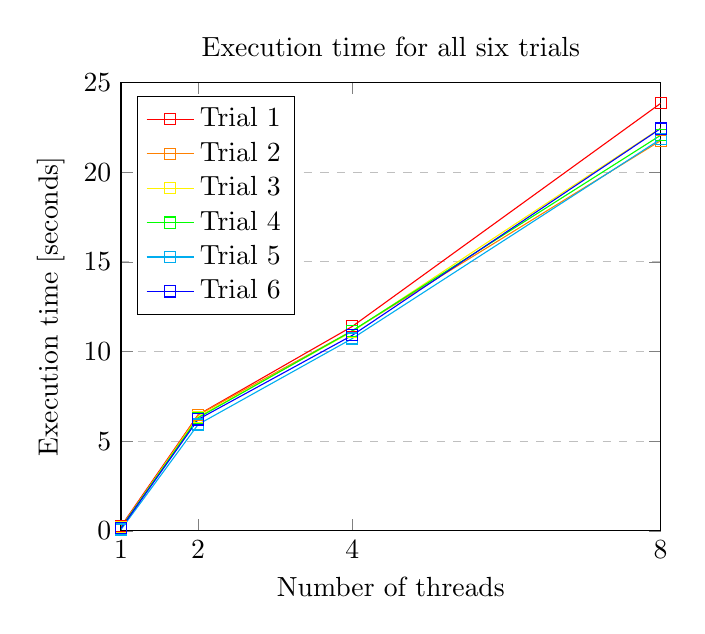
\begin{tikzpicture}
	\begin{axis}[
	    title={Execution time for all six trials},
	    xlabel={Number of threads},
	    ylabel={Execution time [seconds]},
	    xmin=1, xmax=8,
	    ymin=0, ymax=25,
	    xtick={1,2,4,8},
	    ytick={0, 5, 10, 15, 20, 25},
    	legend pos=north west,
	    ymajorgrids=true,
	    grid style=dashed,
	]
	
	% Distribution 1
	\addplot[
	    color=red,
	    mark=square,
	    ]
	    coordinates {
	    %0.2487	6.4415
	    (1, 0.253422)(2, 6.470939)(4, 11.397211)(8, 23.836776)
	    };
    %\legend{Distribution 1}
    
    % Distribution 2
	\addplot[
	    color=orange,
	    mark=square,
	    ]
	    coordinates {
	    %0.2487	6.4415
	    (1, 0.123798)(2, 6.456186)(4, 11.154437)(8, 21.758258)
	    };
    %\legend{Distribution 2}  
    
        % Distribution 3
	\addplot[
	    color=yellow,
	    mark=square,
	    ]
	    coordinates {
	    %0.2487	6.4415
	    (1, 0.191336)(2, 6.357836)(4, 11.117342)(8, 22.457724)
	    };
    % \legend{Distribution 3}
 
	% Distribution 4
	\addplot[
	    color=green,
	    mark=square,
	    ]
	    coordinates {
	    %0.2487	6.4415
	    (1, 0.176446)(2, 6.304448)(4, 11.154646)(8, 22.058291)
	    };
    % \legend{Distribution 4}
 	
 	\addplot[
	    color=cyan,
	    mark=square,
	    ]
	    coordinates {
	    %0.2487	6.4415
	    (1, 0.074183)(2, 5.929456)(4, 10.723320)(8, 21.841913)
	    };
 	
	
	 \addplot[
	    color=blue,
	    mark=square,
	    ]
	    coordinates {
	    %0.2487	6.4415
	    (1, 0.143335)(2, 6.211829)(4, 10.902162)(8, 22.432596)
	    };
 	
 	\legend{Trial 1, Trial 2, Trial 3, Trial 4, Trial 5, Trial 6}
	\end{axis}
	

	
	\end{tikzpicture}
	%\label{Test figure}
\end{figure}


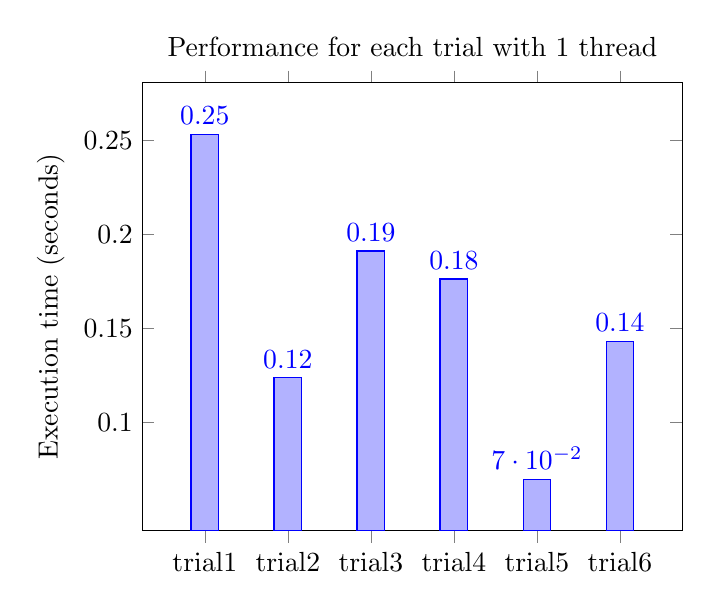
\begin{tikzpicture}
\begin{axis}[
    ybar,
    enlargelimits=0.15,
    legend style={at={(0.5,-0.15)},
      anchor=north,legend columns=-1},
    title={Performance for each trial with 1 thread},
    ylabel={Execution time (seconds)},
    symbolic x coords={trial1,trial2,trial3,trial4,trial5, trial6},
    xtick=data,
    ytick={0,0.1,0.15,0.2,0.25},
    nodes near coords,
    nodes near coords align={vertical},
    ]
\addplot coordinates {(trial1,0.253422) (trial2, 0.123798) (trial3,0.191336)(trial4,0.176446)(trial5,0.07)(trial6,0.143335)};
\end{axis}	
\end{tikzpicture}

\hfill\\

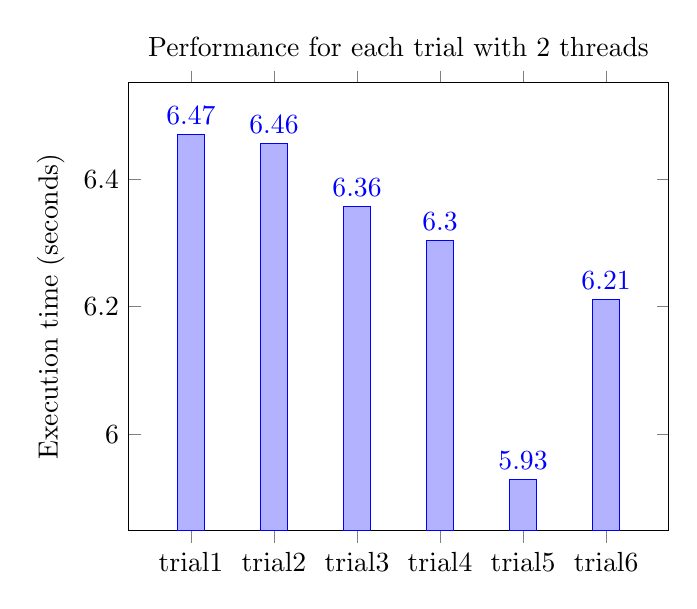
\begin{tikzpicture}
\begin{axis}[
    ybar,
    enlargelimits=0.15,
    legend style={at={(0.5,-0.15)},
      anchor=north,legend columns=-1},
    title={Performance for each trial with 2 threads},
    ylabel={Execution time (seconds)},
    symbolic x coords={trial1,trial2,trial3,trial4,trial5, trial6},
    xtick=data,
    nodes near coords,
    nodes near coords align={vertical},
    ]
\addplot coordinates {(trial1, 6.470939) (trial2, 6.456186) (trial3,6.357836)(trial4,6.304448)(trial5,5.929456)(trial6,6.211829)};
\end{axis}	
\end{tikzpicture}

\hfill\\
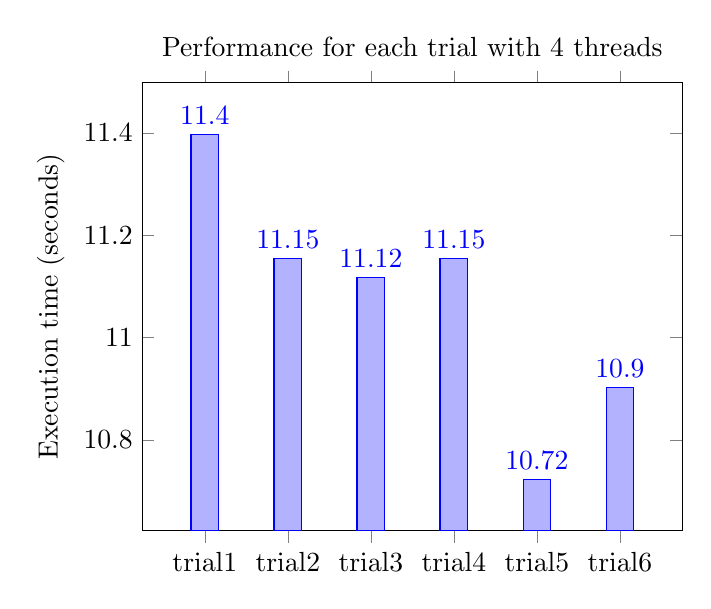
\begin{tikzpicture}
\begin{axis}[
    ybar,
    enlargelimits=0.15,
    legend style={at={(0.5,-0.15)},
      anchor=north,legend columns=-1},
    title={Performance for each trial with 4 threads},
    ylabel={Execution time (seconds)},
    symbolic x coords={trial1,trial2,trial3,trial4,trial5, trial6},
    xtick=data,
    nodes near coords,
    nodes near coords align={vertical},
    ]
\addplot coordinates {(trial1, 11.397211) (trial2,  11.154437) (trial3, 11.117342)(trial4, 11.154646)(trial5, 10.723320)(trial6, 10.902162)};
\end{axis}	
\end{tikzpicture}

\hfill\\

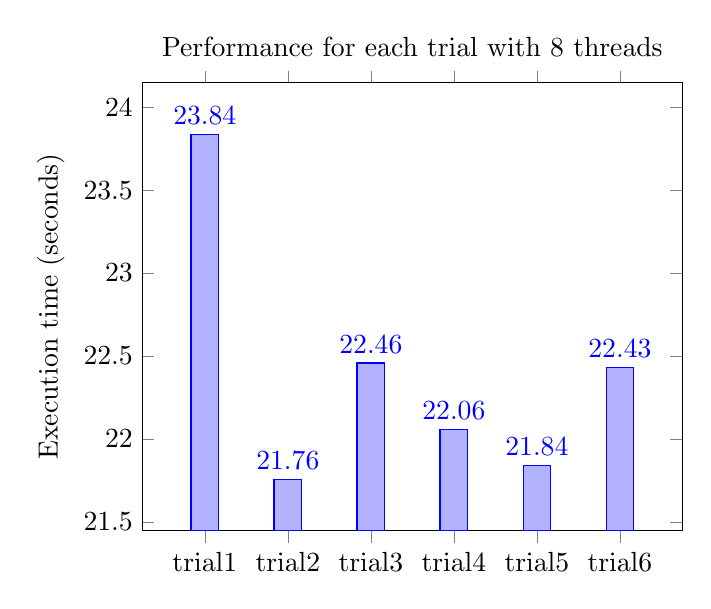
\begin{tikzpicture}
\begin{axis}[
    ybar,
    enlargelimits=0.15,
    legend style={at={(0.5,-0.15)},
      anchor=north,legend columns=-1},
    title={Performance for each trial with 8 threads},
    ylabel={Execution time (seconds)},
    symbolic x coords={trial1,trial2,trial3,trial4,trial5, trial6},
    xtick=data,
    nodes near coords,
    nodes near coords align={vertical},
    ]
\addplot coordinates {(trial1, 23.836776) (trial2,  21.758258) (trial3, 22.457724)(trial4, 22.058291)(trial5, 21.841913)(trial6, 22.432596)};
\end{axis}	
\end{tikzpicture}

\hfill\\

For each graph, we can see that trial 5 took considerably less time for each test with all the different thread possibilities. Consulting Table 1, we can see that thread 5 has the least insertion likelihood. A low time is also noticeable for trial 2 on the 1-thread and 8-thread graphs. Our interpretation is that insertion into our table is the most expensive operation, at least in this initial sequential implementation. Judging by the high results of trials without any contains operations, we feel this is evidence of contains() being the least expensive operation.

It will be interesting to see the affect of the next step in this project: implementing the non-sequential data structure. We expect the final non-blocking hashtable, as originally described, should severely decrease the execution time of our results. The nice thing about our execution C++ code is that they implement the class in a generic fashion, so that we can modify the hashtable code and test against the exact same execution time code.



\section{Analysis and Conclusion}

The non-blocking hashtable proposed by Chris Purcell and Tim Harris uses a number of operations and specialized data types to achieve atomicity non-blocking functionality.  To make our implementation sequential, we were able to simplify the internal structure of the hashtable by eliminating these features and only allowing one thread to modify the hashtable at a time. Though this differentiates it from the proposed implementation and is not non-blocking, it maintains the same hashtable open addressing functionality with the use of probe scanning phases. The result is a sequential version of the proposed hashtable structure.


\ifCLASSOPTIONcaptionsoff
  \newpage
\fi



\begin{thebibliography}{1}

\bibitem{IEEEhowto:kopka}

C.~Purcell and T.~Harris, \emph{Non-blocking Hashtables with Open Addressing}.\hskip 1em plus
  0.5em minus 0.4em\relax Springer-Verlag, Berlin, Heidelberg, 2005.

\end{thebibliography}

\end{document}

